\section{STM32F411CEU6} \label{section:STM32F411CEU6}
\subsection{Why this MCU?} \label{subsection:Why_this_MCU}
The selection of the STM32F411CEU6 was driven by a desire to explore alternatives to the Pi Zero commonly used in similar projects. As pioneers in adopting this microcontroller, we are venturing into uncharted territory.
% Delving into the intricacies of our decision, let's explore the schematic in \autoref{fig:Blackpill_STM32F411CEU6_Schematic}.
\begin{figure}[H]
    \centering
    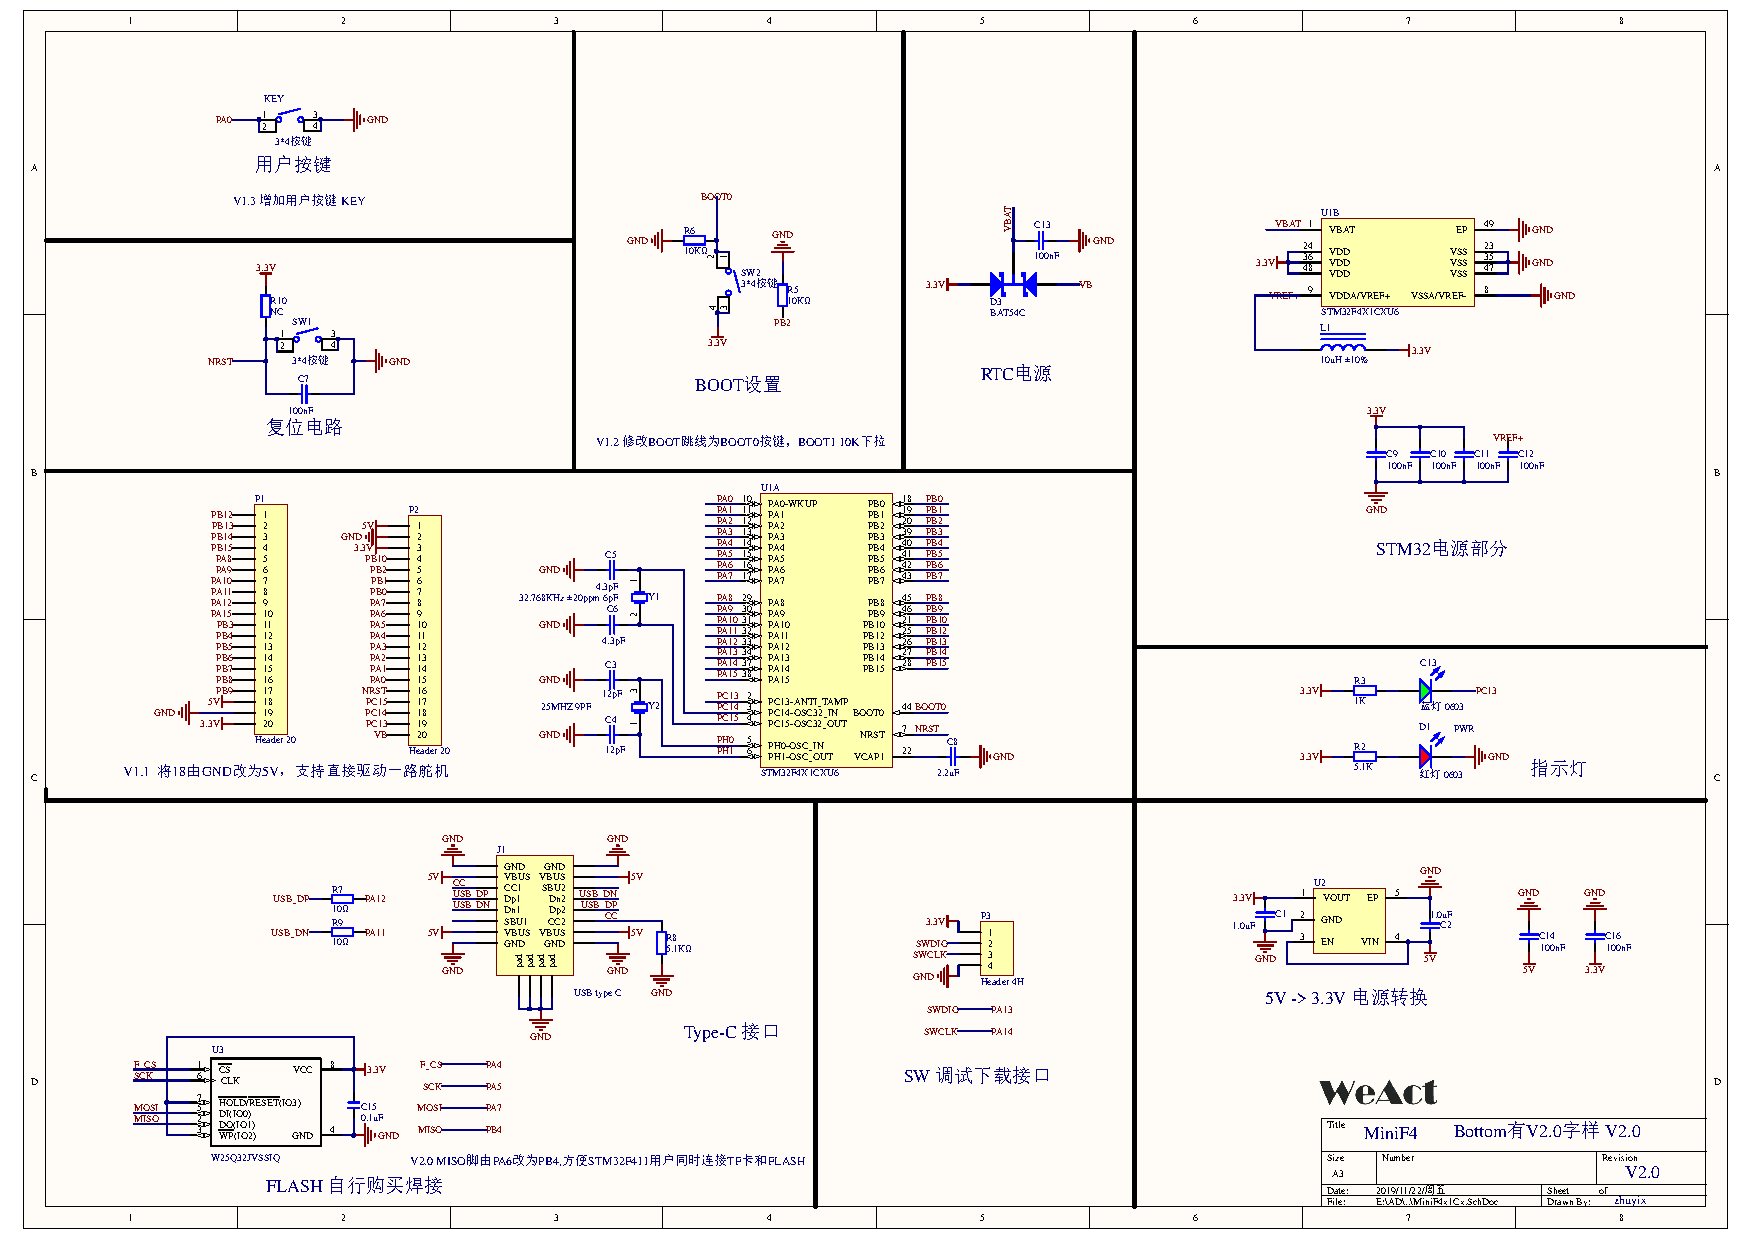
\includegraphics[width=1\linewidth]{img//blackpill/original-schematic-STM32F411CEU6_WeAct_Black_Pill_V2.0.pdf}
    \caption{Blackpill STM32F411CEU6 Schematic}
    \label{fig:Blackpill_STM32F411CEU6_Schematic}
\end{figure}
\begin{itemize}
    \item \textbf{Circuit with Buttons:} The schematic reveals a carefully designed circuit accommodating essential buttons - Key, Switch, and Boot - not crucial since we aren't using the onboard bootloader.

    \item \textbf{Real-Time Clock (RTC):} A dedicated circuit for real-time clock functionality ensures precise timing and synchronization within our motor control system.

    \item \textbf{STM32F411CEU6 Pinout:} The MCU itself is dissected with a pinout, providing insights into the connections and functionalities of each pin.

    \item \textbf{Voltage Regulator:} The presence of a voltage regulator ensures stable and reliable power distribution throughout the system.

    \item \textbf{Additional Circuits:} Beyond these components, the schematic highlights several other circuits vital for the holistic functionality of our design.
\end{itemize}

Moving from the abstract schematic to the tangible layout, the dimensions in \autoref{fig:Blackpill_STM32F411CEU6_Dimensions} depict the spatial arrangement of each component. Assembled into a cohesive unit, the complete PCB with the integrated STM32F411CEU6 is visualized in \autoref{fig:Blackpill_STM32F411CEU6_Picture}.
\begin{figure}[H]
    \centering
    \begin{subfigure}{0.48\textwidth}
        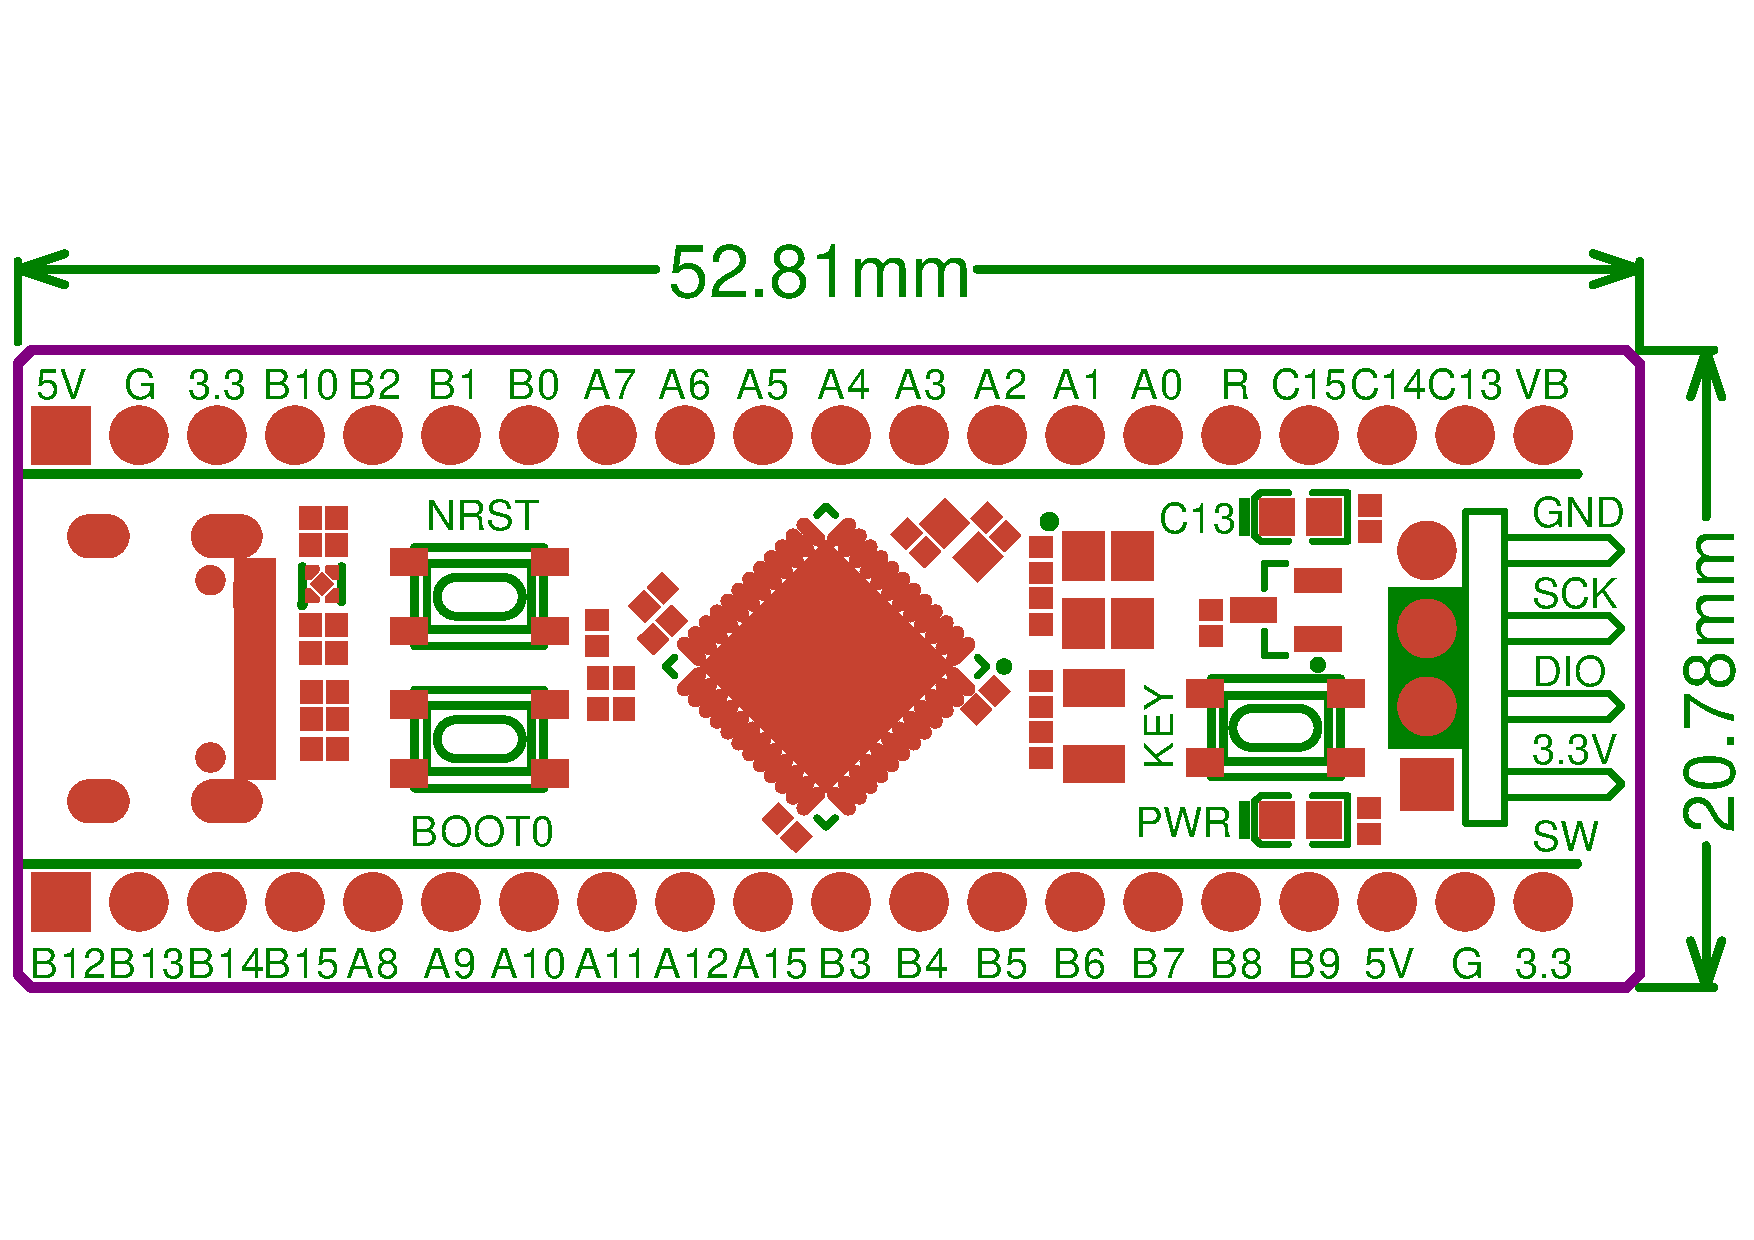
\includegraphics[width=\linewidth]{img/blackpill/original-dimensions-STM32F411CEU6_WeAct_Black_Pill_V2.0.pdf}
        \caption{Blackpill STM32F411CEU6 Dimensions}
        \label{fig:Blackpill_STM32F411CEU6_Dimensions}
    \end{subfigure}
    \hfill
    \begin{subfigure}{0.48\textwidth}
        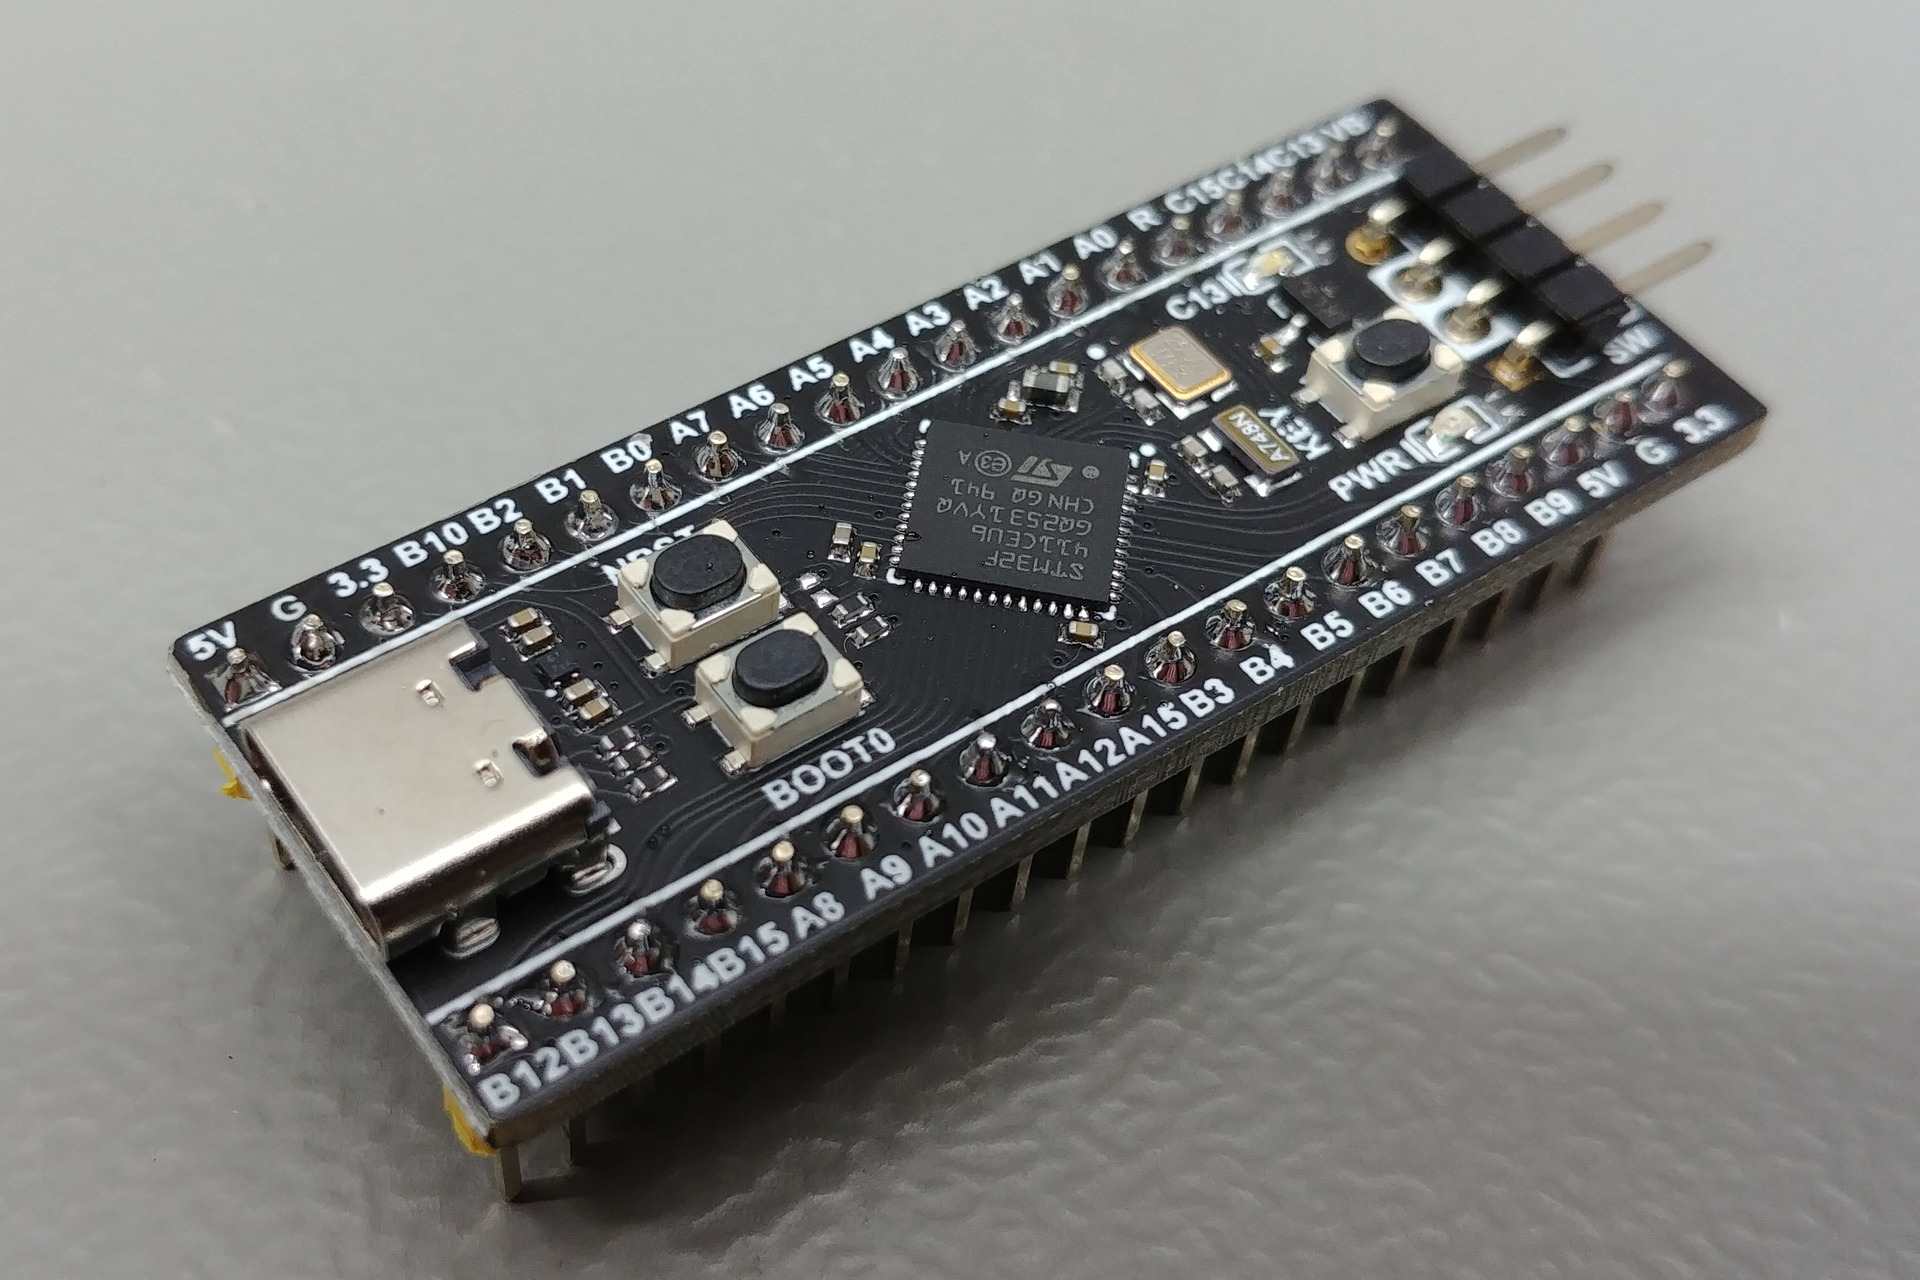
\includegraphics[width=\linewidth]{img/blackpill/STM32F411CEU6_WeAct_Black_Pill_V2.0-1.jpg}
    \caption{Blackpill STM32F411CEU6 Picture}
    \label{fig:Blackpill_STM32F411CEU6_Picture}
    \end{subfigure}
      \caption{Blackpill STM32F411CEU6}
  \label{fig:Blackpill STM32F411CEU6}
\end{figure}
In order to facilitate integration into our PCB design software, footprints and 3D models were developed for the component. Initially, KiCad was chosen for designing the model (see Figure \ref{fig:KiCadModel}) and footprint (see Figure \ref{fig:KiCadFootprint}), owing to our familiarity with the software. Subsequently, following consultation with Ad van den Bergh\cite{Adje}, we transitioned to using Altium Designer (refer to Figure \ref{fig:AltiumModel} \& \ref{fig:AltiumFootprint}). The creation of these models allows for seamless incorporation of the Blackpill breakout board into our custom PCB design.


\begin{figure}[H]
    \centering
    \begin{subfigure}{0.2\textwidth}
        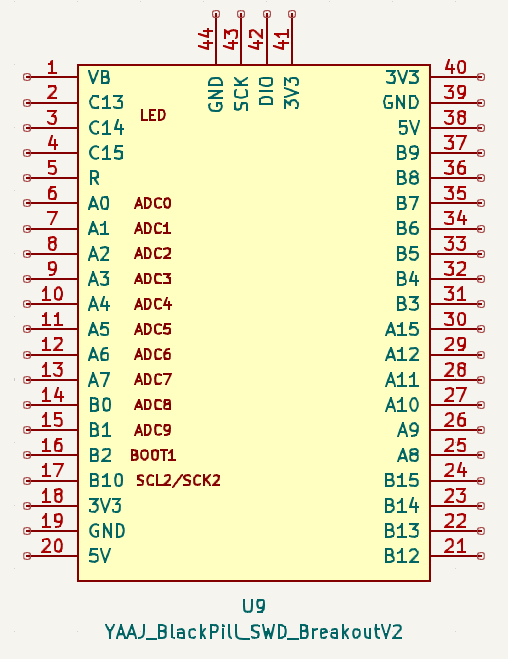
\includegraphics[width=\linewidth]{img//blackpill/KiCadMODEL.png}
        \caption{KiCad Model}
        \label{fig:KiCadModel}
    \end{subfigure}
    \hfill
    \begin{subfigure}{0.1\textwidth}
        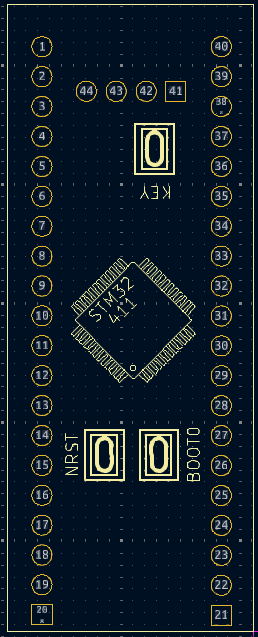
\includegraphics[width=\linewidth]{img//blackpill/KiCadFOOTPRINT1.png}
    \caption{KiCad Footprint}
    \label{fig:KiCadFootprint}
    \end{subfigure}
        \hfill
    \begin{subfigure}{0.2\textwidth}
        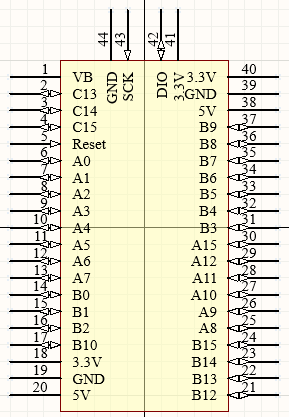
\includegraphics[width=\linewidth]{img//blackpill/AltiumMODEL.png}
        \caption{Altium Model}
        \label{fig:AltiumModel}
    \end{subfigure}
    \hfill
    \begin{subfigure}{0.2\textwidth}
        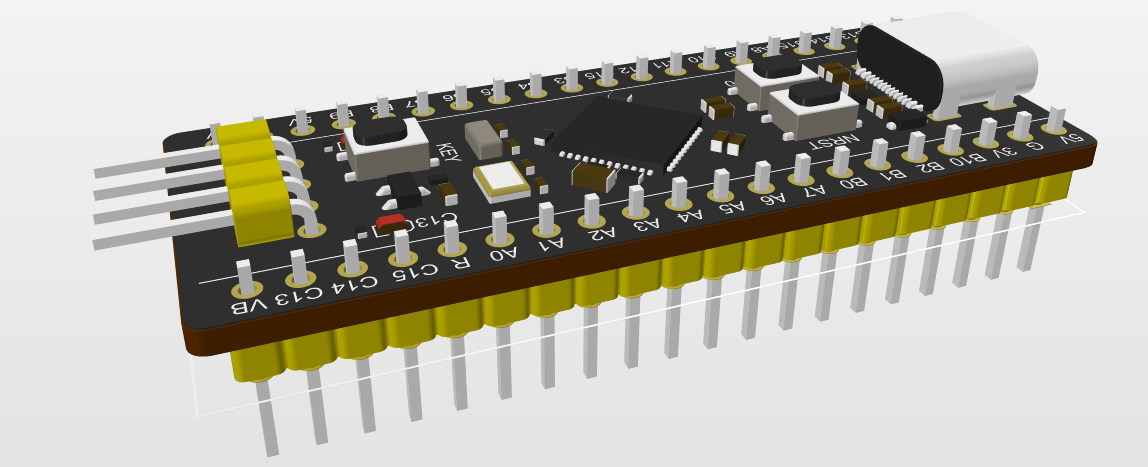
\includegraphics[width=\linewidth]{img//blackpill/AltiumFOOTPRINT.png}
    \caption{Altium Footprint}
    \label{fig:AltiumFootprint}
    \end{subfigure}
      \caption{Models\&Footprints}
  \label{fig:KiCadPCB}
\end{figure}


